%%%%%%%%%%%%%%%%%%%%%%%%%%%%%%%%%%%%%%%%%%%%%%%%%%%%%%%%%%%%%%%%%%%%%%%%%%%%%%%%%%%%%%%%%%%%%
%%									Chapitre 1											%
%%%%%%%%%%%%%%%%%%%%%%%%%%%%%%%%%%%%%%%%%%%%%%%%%%%%%%%%%%%%%%%%%%%%%%%%%%%%%%%%%%%%%%%%%%%%%
\chapter{Théorie sur le calendrier Potager}
	\minitoc
	\newpage
%%%%%%%%%%%%%%%%%%%%%%%%%%%%%%%%%%%%%%%%%%%%%%%%%%%%%%%%%%%%%%%%%%%%%%%%%%%%%%%%%%%%%%%%%%%%%
% Début du chapitre
\section{Définition du potager}
 Un potager est une parcelle de terrain généralement réservée à la culture de légumes, de fruits, d'herbes aromatiques et parfois de fleurs comestibles, dans le but de fournir une source de nourriture fraîche pour une famille ou une communauté. Les potagers peuvent varier en taille, allant de petits espaces dans les arrière-cours urbaines à de vastes champs ruraux. Le calendrier du potager vise à maximiser le rendement des cultures en les alignant avec les conditions idéales pour leur croissance. Certains calendriers se basent sur des méthodes traditionnelles, tandis que d'autres intègrent des données scientifiques modernes pour fournir des recommandations précises. \\
 Un potager est un espace spécialement aménagé où l'on cultive une variété de légumes, d'herbes aromatiques et parfois de fruits pour la consommation personnelle. Il s'agit d'un jardin productif conçu pour la culture de plantes comestibles, offrant ainsi un approvisionnement de produits frais et locaux pour une alimentation saine et durable. Ce petit coin de terre, soigneusement entretenu, permet de cultiver une diversité de végétaux, favorisant l'autosuffisance alimentaire tout en étant un lieu de connexion avec la nature et d'apprentissage sur la croissance des plantes.\\
L'objectif global d'un calendrier de potager est d'optimiser la production, la santé et la qualité des cultures tout en respectant les cycles naturels. Cela peut contribuer à une gestion plus durable des ressources et à une meilleure compréhension des interactions entre la nature et l'agriculture.\\
Il va donc nous accompagner mois par mois pour savoir :\\
\begin{itemize}
	\item[-]quelle variété choisir et quand planter ,
	\item[-]quand effectuer les semis du potager.
\end{itemize}
C'est donc un tableau de bord pour cultiver votre potager.
\subsection{Rotation des cultures et disposition des différentes espèces}
La rotation des cultures et la disposition des différentes espèces sont des pratiques agricoles visant à optimiser la santé du sol, à prévenir les maladies et les ravageurs, et à améliorer le rendement des cultures. Voici ce que ces pratiques impliquent :
\subsubsection{Rotation des cultures : } La rotation des cultures consiste à alterner les types de cultures cultivées sur une parcelle de terrain au fil des saisons ou des années. Cette rotation vise à éviter l'épuisement des nutriments spécifiques du sol et à réduire le risque de maladies et de ravageurs qui se développent souvent lorsque les mêmes plantes sont cultivées de manière continue. En alternant les cultures, certaines plantes peuvent même aider à rétablir ou à maintenir l'équilibre des nutriments dans le sol. Par exemple, une culture peut ajouter des nutriments au sol tandis qu'une autre peut en prélever davantage.
\subsubsection{ Disposition des différentes espèces : }La disposition des différentes espèces fait référence à la manière dont différentes plantes sont arrangées dans un jardin ou un champ. Il peut s'agir de la disposition spatiale des cultures ou de la manière dont différentes espèces de plantes sont regroupées. Cette disposition peut avoir des avantages synergiques, tels que la lutte contre les ravageurs, la promotion de la biodiversité, et la maximisation de l'utilisation des ressources.
Par exemple, certaines plantes ont des propriétés répulsives pour les insectes nuisibles à d'autres plantes. En les plantant à proximité, on peut réduire le besoin de pesticides. De plus, certaines plantes peuvent avoir des besoins en nutriments différents ou peuvent être complémentaires dans la manière dont elles exploitent les ressources du sol.\\
En résumé, la rotation des cultures et la disposition des différentes espèces sont des pratiques agricoles stratégiques visant à promouvoir la santé du sol, à prévenir les problèmes liés à la monoculture et à améliorer la durabilité globale de l'agriculture.
\section{Documentation du projet}
Dans le cadre de cette mémoire on a demandé l’avis des techniciens d’un groupe spécialisé dans la culture appeler "Union Matanjaka".\\
L'Union Matanjaka est une organisation paysanne née de l'initiative de leaders paysans du district de Diego II qui œuvre depuis 2003 pour le développement rural des Districts de Diego II et de Diego I.\\
On nous  propose  pour  simplifier  la tâche  que pour les deux premières années, les mises en culture proposées par le cycle simple décrit sont regroupées en deux périodes clefs pour chacune des deux années du cycle :
\begin{itemize}
\item[-]Grande saison qui se trouve entre le mois Octobre/Novembre  jusqu’à Mars/Avril.\\
c'est une saison chaude favorable à la culture du riz
\item[-]Contre saison qui se trouve entre le mois Mars/avril jusqu’en  octobre /Novembre		
\end{itemize}
On va parler de la contre saison,elles ont l’avantage de convenir quasiment à tous les climats.
Pour la culture on peut donc par exemple suivre cette étape.
\begin{itemize}
\item[-]Octobre : préparation du sol (labour, fumure,…)
\item[-]Novembre/décembre : semis
\item[-]Et après, les pépinières après  2 semaine on peut déjà repiquer/transplanter.
\item[-]Entretien : après 3 ou 4 mois on est dans la saison de récolte
\end{itemize} 
Apres récolte on reprend le système de culture contre saison.Donc par exemple:\\
si on a cultivé avant des cultures de la famille des graminées pour entretenir et garder la fraicheur et les minéraux du sol on cultive les cultures de la famille des légumineuses. On recommence à semer on change de famille.\\
Ou encore on a,si on cultive des pomme de terre  on ne peut pour la culture suivante, cultiver des tomate car il appartienne tous dans la famille de Solanacées, tout ceci est dans un régime ou on a constamment de l’eau.
Les pommes de terre ne peut germer a + de 28ºC.\\
Voici une représentation du calendrier de potager
%%%%%%%%%%%%%%%%%%image_de_calendrier_potager%%%%%%%%%%%%%%%%%%%
%%%%%%changer cette image
	\begin{figure}[!h]
    	\center
    		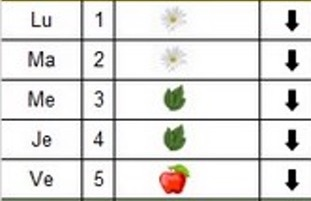
\includegraphics[width=0.3\textwidth]{image/image_de_calendrier_potager2.jpg}
   		\caption{Calendrier potager}
    	\label{calendrier potager}
	\end{figure}
%%%%%%%%%%%%%%%%%%%%%
Le calendrier définit les potages on 4 grande famille.
\begin{itemize}
\item[-]fruitier : pomme
\item[-]en raciner : pomme de terre 
\item[-]fleuri : choux fleur
\item[-]feuiller : salade
\end{itemize} 
Il existe plusieurs bande dans le calendrier.
\begin{itemize}
\item[-]bande rouge : entretien/repiquage
\item[-]bande blanche : semi ex : riz tomate, (grain)
\item[-]Zone colore : interdit semi
\end{itemize} 
\subsection{Biodynamique}
La biodynamie est une approche agricole holistique qui considère la ferme comme un organisme autonome, interconnecté avec les forces cosmiques et terrestres. Cette méthode a été développée au début du 20e siècle par le philosophe autrichien Rudolf Steiner. La biodynamie intègre des pratiques agricoles organiques avec des éléments ésotériques et spirituels, et elle accorde une attention particulière aux cycles lunaires et planétaires.\\
Voici comment la biodynamie est liée à la rotation des cultures et à la disposition des différentes espèces :\\
    \subsubsection{Calendrier biodynamique :} Les praticiens de la biodynamie suivent un calendrier spécifique basé sur les positions des planètes et des étoiles. Ce calendrier influence les activités agricoles, y compris la rotation des cultures. Selon la biodynamie, certaines phases lunaires ou positions planétaires peuvent influencer la croissance des plantes et le développement du sol. Les périodes favorables ou défavorables peuvent être prises en compte pour planifier la plantation, la récolte et d'autres activités agricoles.\\
   \subsubsection{Préparations biodynamiques : }La biodynamie utilise également des préparations spéciales, souvent élaborées à partir de plantes, de minéraux et de compost, qui sont appliquées au sol ou aux cultures pour renforcer la vitalité de la ferme. Ces préparations sont souvent utilisées en association avec des événements cosmiques spécifiques, tels que les éclipses ou les phases lunaires particulières.\\
    \subsubsection{Rotation des cultures et dynamique des plantes :  } La biodynamie encourage une rotation des cultures qui prend en compte les forces cosmiques et la dynamique spécifique de chaque plante. Certains praticiens peuvent également mettre en œuvre des principes de compagnonnage des plantes, où des plantes spécifiques sont associées pour favoriser la croissance mutuelle et la santé du jardin.\\
    \subsubsection{Observation des rythmes naturels :} Les agriculteurs biodynamiques sont encouragés à observer attentivement les rythmes naturels et à ajuster leurs pratiques agricoles en conséquence. Cela inclut non seulement les cycles lunaires, mais aussi d'autres cycles cosmiques et terrestres.\\
Donc on a dressé un tableau qui retrace la liste de la culture possible à Diego Suarez (Antsiranana).

\begin{table}[!h]
\caption{La liste de la culture}
\label{La liste de la culture}
\begin{center}
\begin{tabular}{|c|c|c|c|}
\hline 
Désignation & Cycle de végétation & Période Favorable & Période de récolte \\ 
\hline 
Arachide &  &  &  \\ 
\hline 
Aubergine & & Mars-Avril/Aout-septembre  &Mois après semi  \\ 
\hline
Betterave & 100-130 jours & Septembre-décembre &  \\ 
\hline 
Carotte &3-4 mois &  & 70-85 jours après semi \\ 
\hline 
Chou de chine & 3 mois &  & 2-3 mois \\ 
\hline
Chou de brocoli & 5-6 mois &  &  \\ 
\hline
Chou-fleur & 6-7mois &  & 6 mois après repiquage \\ 
\hline 
Chou &3-3 ½  mois & Février-Juillet &  2 ½  mois après\\ 
\hline
Concombre & 3 mois &  & 3 mois \\ 
\hline 
Courge & 4-5 mois &  &  \\ 
\hline
Courgette & 2 mois &  &  \\ 
\hline
Gingembre & 9-10 mois &  &  \\ 
\hline 
Haricot sec & &  & 120-130 jours \\ 
\hline 
Haricot vert & &  & 50 jours  \\ 
\hline
Laitue & 70-90 jours &  &  \\ 
\hline
Melon & &  &  \\ 
\hline 
Navet & &  &  \\ 
\hline
oignons & 120-170 jours &Mai - septembre  &  \\ 
\hline 
Petit pois &70-100 jours & Avril- Aout  &  \\ 
\hline 
persil & 5-6 mois &  &  \\ 
\hline
poireau & &  &4-6 mois après semis  \\ 
\hline
Piment  & 5-6 mois &  &  \\ 
\hline
Pois de cap & & Mars-septembre &  \\ 
\hline 
Poivron & 3-6 mois & Mars – juillet & 3 mois après semis  \\ 
\hline
Pomme de terre & 5-6 mois &  &  \\ 
\hline 
Radis &  &  &  \\ 
\hline 
Sojas & &  &  \\ 
\hline
Tomate & &  &  3 mois après semis\\ 
\hline
\end{tabular}
\end{center} 
\end{table} 
\subsection{Utilisation du calendrier potager} 
Pour utiliser le calendrier il faut savoir le type de fructification de la plante que l’on veut cultiver. Pour  choisir la période correspondant.\\
La conception biodynamique du jardinage et de l’agriculture est basée sur la nécessiter de concevoir  le domaine  agricole  ou jardinage comme un organisme vivante.\\

La plante à la différence de l’animal ou du genre humain est totalement ouvert à son environnement .Les différent rythme du cosmos comme le rythme du soleil, lune et….. Influence beaucoup les plantes.Mais là la question se pose, comment  détecter ces influence de ses rythme dont on ne fait pas l’expérience directe ?\\Pour répondre à cette question la chercheuse allemand  Maria  Thun, à la suite  de quelque  prédécesseur  comme Lily kolisko  et Frantz  Rulini, depuis une cinquantaine d’année. Étudiant la croissance de plante et les moments de semis.\\

Le calendrier de semis  peut aider  à choisir  des  dates favorables ou à éviter  des dates  défavorables ,mais  c’est  aussi  un outils de travail pour s’ouvrir au nombreux rythme  cosmique  et apprendre  a toujours  mieux  ressentir l’instant présent  en développant  son sens  de l’observation.\\
La plante vive en total dépense au rythme des journées, des mois et de l’année.Il ne prend pas seulement en compte les positions de la lune, mais aussi celle des planètes du système solaire et leur configuration.
En Afrique, chaque année, la végétation s'éveille pendant la saison des pluies, s'épanouit sous le soleil de l'été et mûrit lors de la saison sèche, qui est généralement en hiver. \\
%%%%%%%% a revoire
\section{Rythme de la lune}
Tout comme le soleil, la lune peut faire beaucoup de bien à votre jardin. En effet, notre satellite imprime son rythme à la nature. Jardiner avec la lune, c’est donc également cultiver ses végétaux en harmonie avec la terre.\\
Comme nous l’avons dit les plantes dépendent de nombreux facteur comme la lune. On va don essayer d’étudier le rythme de se dernier.

\subsection{Rythme synodique}
A un certain moment, le soleil est opposée  a la lune par rapport à la terre, l’éclaire en pleine face : c’est la pleine lune.\\
A d’autre moment, il est on conjonction avec la lune, c’est-à-dire qu’il est derrière la lune vue de la terre. La lune est alors totalement invisible, c’est la nouvelle lune.\\
%%%%%%%%%%%%%image_rythme_synodique%%%%%%%%%%%%%%%%%%%%%%%
\begin{figure}[!h]
    	\center
    		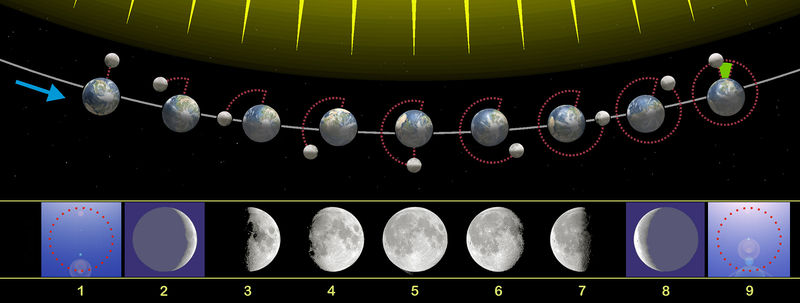
\includegraphics[width=0.8\textwidth]{image/Moon_phases_00}
   		\caption{Rythme synodique}
    	\label{Rythme synodique}
	\end{figure}

On a donc une durée de la position de lune croissante à décroissante 29.5 jours avec 15 jours croissante et 15 jours décroissants.\\
Avec un mouvement de la pleine lune vers la nouvelle lune ou  période veille.
\subsection{Rythme sidéral}
Il y aussi le rythme sidéral devant les signes de zodiaque durée 27.3 jours. En effectuant sa rotation autour de la terre, chaque mois, la Lune passe devant les 12 constellations du zodiaque comme le fait le soleil en un an. Le rythme sidéral est la période qui sépare deux passages successifs de la Lune devant le même groupe d'étoiles (d'où l'adjectif sidéral) du zodiaque.\\
L'utilisation de ce rythme a été popularisée par Maria Thun qui a procédé à des semis journaliers de radis en sol pauvre et sans irrigation. Celle-ci aurait constaté des variations morphologiques, avec des parties de la plante plus ou moins stimulées selon le jour concerné, et donc la constellation du zodiaque du moment du semis.\\
Inversement les plantes appartiennent à l'une ou l'autre de ces catégories selon la partie de la plante utilisée : il convient alors de les semer et de les soigner préférentiellement aux dates feuille, fruit, fleur ou racine.
%%%%%%texte A revoire
\\
%%%%%%%%%%%%%image rythme sidéral%%%%%%%%%%%%%%%%%%%%%%%
\begin{figure}[!h]
    	\center
    		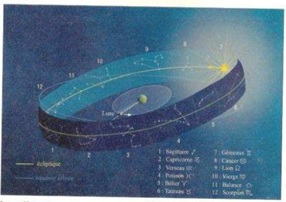
\includegraphics[width=0.5\textwidth]{image/sideral}
   		\caption{Rythme sidéral}
    	\label{Rythme sidéral}
	\end{figure}
\subsection{Les phases de la Lune}
Un cycle lunaire est constitué des phases de la Lune : Nouvelle lune, Premier croissant, Premier quartier, Lune Gibbeuse, Pleine lune, de nouveau Lune Gibbeuse, Dernier quartier, Dernier croissant.\\

Les phases de la Lune correspondent à ses portions illuminées par le soleil qui sont visibles de la Terre. La Lune tournant en orbite autour de la Terre, ces portions ne cessent de changer en fonction de la position de l'astre.\\

Un cycle lunaire est aussi appelé une lunaison \\
Comme nous l’avons dit les plantes dépendent de nombreux facteur comme la lune. On va donc essayer d’étudier le rythme de se dernier.\\
Les différentes phases de la Lune ont des noms différents.\\
Alors que la Lune est croissante, c'est-à-dire que la proportion de sa surface illuminée visible depuis la Terre augmente, et que sa position dans le ciel observé à minuit, parcourt le ciel d'ouest en est en deux semaines, les phases sont :
 \begin{itemize}
\item[-]la nouvelle lune , la Lune se situe en conjonction avec le Soleil. Elle n'apparaît pas dans le ciel de nuit, mais en journée et présente sa face obscure à la Terre, ce qui la rend difficilement observable ;
\item[-]le premier croissant , qui correspond à sa réapparition dans le ciel nocturne ;
\item[-]premier quartier , elle est en quadrature et a la forme d'un D ;
\item[-]la pleine lune , elle est maintenant en opposition et totalement éclairée par le Soleil. Si on observe bien on peut observer les mers (ce sont les taches sombres qui sont en fait des restes de lave qui se sont écoulées sur la Lune).
 \end{itemize}
%%%%%%%%image rytme de la lune%%%%%%%%%%%%%%%
\section{Calcule des phases lunaires}
Le calendrier dépend entièrement généralement du rythme de la lune. On va donc essayer de savoir les différentes phases.
Par définition, les heures de la Maintenant Lune, du Premier Quartier, de la Pleine Lune et du Dernier
Quartier sont les heures auxquelles l'excédent de la longitude apparente de la Lune sur la longitude apparente
du Soleil est respectivement de 0°, 90°, 180° et 270°.\\
Ainsi, pour calculer les Instants de ces phases lunaires, il faut calculer les
longitudes apparentes de la Lune et du Soleil séparément. (cependant, l'effet de la nutation peut
être négligé ici, puisque la nutation, en longitude $\Delta\psi$ n'affectera pas la différence entre les longitudes
de la Lune et du Soleil.)\\
Cependant, si aucune grande précision n'est requise, les instants des phases lunaires peuvent être
calculé selon la méthode décrite dans ce chapitre. Les expressions sont basées sur la théorie
ELP­2000/82 de Chapront pour la Lune (avec des expressions améliorées pour les arguments M,
M', etc., comme mentionné au chapitre 45), et sur la théorie VSOP87 de Bretagnon et Francou
pour le Soleil. Les temps résultants seront exprimés en Jours Éphémérides Juliens (JDE), donc en
Temps Dynamique.\\
Cet algorithme calcule la nouvelle Lune du début d’un cycle lunaire. Donc si la nouvelle lune est vers la fin du mois les phases chevaucheront deux mois. Ce qui est le cas pour Avril 2009. Les phases sont en Avril et Mai 2009.  Du 25 Avril au 20 Mai. Donc pour certain mois comme 2003-03 le cycle lunaire commence le 2003-04 et non le 2003-03.\\
Comme on l’a dit on a besoin de deux valeurs d’entrée A pour année et Mo pour mois.Et des divers anomalie M pour trouver les diverses phases lunaires. Pour bien comprendre on va donner la valeur A=2017 et Mo=6. \\
On calcul k avec une coefficient 12.3685 une constant pour definir une date simple en siecle Julien  qui est:
\[k = (A+ mois – 2000)*12,3685\]
on aura donc :
\[k =215\]
Une valeur entière de k représente le moment de la Nouvelle Lune. Pour déterminer d'autres phases lunaires, on peut ajouter des fractions spécifiques à k. 
\begin{itemize}    
\item[]0,00 pour la Nouvelle Lune Ex:  k = 215
\item[]0,25 pour le Premier Quartier Ex: k = 215,25
\item[]0,50 pour la Pleine Lune Ex: k = 215,5
\item[]0,75 pour le Dernier Quartier Ex: k = 215,75
\end{itemize}
Toute valeur de k autre que celles spécifiquement définies dans ce contexte produira des résultats qui n'ont pas de signification logique ou pratique. En l'occurrence, la valeur est associée à la Nouvelle Lune du 6 janvier 2000. Les valeurs négatives de k sont utilisées pour représenter des phases lunaires antérieures à l'année 2000. Il est important de respecter ces paramètres spécifiés, car des valeurs de k non conformes conduiraient à des conclusions dénuées de sens dans le cadre de cette méthode particulière.\\
Avec les k obtenu on calcule T qui est le temps en siècles juliens depuis l'époque 2000 ; il est obtenu avec une précision suffisante à partir de:
\[T =k \backslash 1236,85  \text{  on alors T = 0,17464}\]
Ensuite en cherche les anomalie moyenne du Soleil au temps et convertir tous les angles que fait la lune par rapport à la terre dans un intervalle 0°-360° grace a la fonction.\\
Les anomalie ou angle moyen du soleil en fonction du temps est:
\[M = 2.5534 + 29,10535669 * k - 0.00000218 x T^{2} - 0,00000011 x T^{3} \]
M = 6289,310444	
Les anomalie ou angle moyenne de la Lune :
\[M’ = 201,5643 + 385,81693528 * k + 0,0107582 * T^{2}+ 0,00001238 * T^{3}- 0,000000058 * T^{4}\]
M' = 83538,0226
L'argument de la latitude de la Lune :
\[F = 160,7108 + 390,67050284 * k - 0,0016118 * T^{2}- 0,00000227 * T^{3}+ 0,00000001 * T^{4}\]
F=84545,5393
Longitude du nœud ascendant de l'orbite lunaire :	
\[\Omega= 124,7746 - 1,56375588  *k + 0,0020672 * T^{2}+ 0,00000215 * T^{2}\]
\Omega = -212,9965897\\
Nous utilisons un total de 14 variables, chacune correspondant à une phase spécifique des cycles lunaires. Chacune de ces variables est soigneusement définie et représente une mesure précise de l'état de la Lune à un moment donné. \\
\begin{landscape}
\begin{table}[!h]
\caption{Les variables de correction}
\label{Les variables de correction}
\begin{center}
\begin{tabular}{|c|c|c|c|c|c|}
\hline 
 & 14 Variables de correction&  NL en[ $^{\circ}$ ] & PL en[ $^{\circ}$ ] & PQ  en[ $^{\circ}$ ]& DQ en[ $^{\circ}$ ] \\ 
\hline 
$A_{1}$ & $299,77 + 0,107408 * k – 0,009173 T2$  & 322,9698482 & 322,916145536444 &  322,889294182478 & 322,942996871906\\ 
\hline 
$A_{2}$ & $ 251,88 + 0,016321 * k $              & 255,405336  & 255,3971755      &  255,39309525   & 255,40125575\\ 
\hline 
$A_{3}$ & $251,83 + 26,651886 * k $              & 6008,63737  & 5995,311433      &  5988,6484615   & 6001,9744045 \\ 
\hline 
$A_{4}$ & $ 349,42 + 36,412478 * k$              & 8214,515248 & 8196,309009      & 8187,2058895    & 8205,4121285 \\ 
\hline 
$A_{5}$ & $ 84,66 + 18,206239 * k $              & 4017,207624 & 4008,1045045     & 4003,55294475   & 4012,65606425 \\ 
\hline 
$A_{6}$ & $141,74 + 53,303771 * k$               & 11655,35454 & 11628,7026505    &11615,37670775   & 11642,02859325\\ 
\hline 
$A_{7}$ & $207,14 + 2,453732 * k $               & 737,146112  & 735,919246       & 735,305813      & 736,532679   \\ 
\hline 
$A_{8}$ & $154,84 + 7,306860 * k $               & 1733,12176  & 1729,46833		  &1727,641615      &1731,295045\\ 
\hline 
$A_{9}$ & $34,52 + 27,261239 * k $               & 5922,947624 & 5909,3170045     &5902,50169475    &5916,13231425\\ 
\hline 
$A_{10}$ & $ 207,19 + 0,121824 * k$              & 233,503984  & 233,443072       & 233,412616       &233,473528 \\ 
\hline 
$A_{11}$ & $291,34 + 1,844379 * k $              & 689,725864  &688,8036745       & 688,34257975     &689,26476925\\ 
\hline 
$A_{12}$ & $161,72 + 24,198154 * k $             & 5388,521264 &5376,422187		  & 5370,3726485      &5382,4717255\\ 
\hline 
$A_{13}$ & $239,56 + 25,513099 * k $             & 5750,389384 &5737,6328345      &5731,25455975     &5744,01110925 \\ 
\hline 
$A_{14}$ & $331,55 + 3,592518 * k $              & 1107,533888  &1105,737629     &1104,8394995        &1106,6357585
\\ 
\hline 
\end{tabular}
\end{center} 
\end{table}
\end{landscape}
Les équations sont fournies par Jean Meeus dans le chapitre 47. Cependant, chaque variable est associée à des facteurs de correction visant à compenser les erreurs. L'équation adopte la forme $x*\sin(variable)$, où les fonctions trigonométriques sont exprimées en radians.\\
Les groupes de correction se répartissent comme suit :
Le premier groupe de facteurs de correction s'applique à toutes les phases lunaires. Pour chacune de ces phases, des facteurs de correction spécifiques sont pris en compte.
\begin{landscape}
\begin{table}[H]
	\caption{ Premier groupe de facteurs de correction}
	\label{ Premier groupe de facteurs de correction}
	\begin{center}
		\begin{tabular}{|c|c|c|c|c|}
\hline 
Équation                    &  résultat pour NL     & résultat pour  PL     & résultat pour  PQ     & résultat pour DQ  \\ 
\hline 
$+0,000325 x \sin A_{1} $   & -0,000195726446451076 & -0,000195969543384474 & -0,000196091027333202 & -0,000195848016479172\\ 
\hline 
$+0,000165  * \sin A_{2} $  & -0,000164911 &-0,00015966996260938&-0,000159666999759314&-0,000159672924649695\\ 
\hline 
$+0,000164 * \sin A_{3} $   & 0,000124787& -0,00013485024979265 & -0,000123109904148533 & -0,000144768995875441\\ 
\hline 
$0,000126  * \sin A_{4} $   & -0,000114641210533772 & -0,000125236904802144 & 0,00441993714893402 & -0,000121468935308566 \\ 
\hline 
$+0,000110 * \sin A_{5} $   & 9,2470254564845E-05 & 8,1880045261142E-05 & 7,57927028433038E-05 & 8,74509416967826E-05\\ 
\hline 
$+0,000062  * \sin A_{6} $ & 4,35685049673676E-05 & 5,87261176018441E-05 & 6,17272086710506E-05& 5,25625792498189E-05\\ 
\hline 
$+0,000060   * \sin A_{7} $ & 1,76885674854124E-05 &1,64569354783273E-05 &1,58382545240628E-05&1,70737300324346E-05\\ 
\hline 
$+0,000056 * \sin A_{8} $ & -5,15016559550923E-05  &-5,279824801507E-05 & 2,86106842219774E-05&-5,21764677534537E-05\\ 
\hline 
$+0,000047 * \sin A_{9} $ & 1,37825513215227E-05 &2,39835221158898E-05&-5,33663647699318E-05&1,90174169348782E-05\\ 
\hline 
$+0,000042 * \sin A_{10} $ & -3,37637251993606E-05  & -3,37371492901123E-05& -3,37238470347936E-05&-3,37504420128866E-05\\ 
\hline 
$+0,000040  * \sin A_{11} $ & -2,01655130139186E-05 & -2,07188860792644E-05&-2,09935687974932E-05 &-2,04428615259341E-05\\ 
\hline 
$+0,000037 * \sin A_{12} $ & -7,36315704146046E-06 & -1,47997836878978E-05&-1,82912047200385E-05&-1,1143527025191E-05\\ 
\hline 
$+0,000035 * \sin A_{13} $ & -5,8433001652702E-06 & -1,33189169430474E-05&-1,68321648305043E-05&-9,6407839056416E-06\\ 
\hline 
$+0,000023 * \sin A_{14} $ & 1,0632282711347E-05 & 9,98776778602614E-06&9,66178942716129E-06&1,03112920451936E-05\\  
\hline 
Somme S1 de ce groupe :& -0,000563270890046784 &-0,000560065256360811&-0,000556294647033336&-0,000562496994576873

\\  
\hline 
		\end{tabular}
	\end{center} 
\end{table}
\end{landscape}
Simultanément, une variable E est calculée en tant que facteur d'ajustement. Cette variable est introduite pour prendre en considération la variation de l'excentricité de l'orbite terrestre autour du Soleil, laquelle évolue au fil du temps. E est utilisée pour moduler les termes dans les équations mathématiques qui dépendent de l'angle M, de manière à refléter cette évolution. Cette variable est exprimée en temps en siècles juliens, ce qui peut donner une valeur négative si la date choisie précède l'époque de l'an 2000.//

Ensuite, les angles suivants, qui sont exprimés en degrés, peuvent être ramenés dans la plage de 0 à 360 degrés, voire convertis en radians si nécessaire, avant de continuer le calcul.
\[E = 1 – 0.002516 * T – 0.0000074 * T^{2}\]
E=0,9995604\\

Il y a les Deuxième groupe de facteurs de correction pour  la nouvelle lune.\\
\begin{table}[H]
	\caption{Deuxième groupe de facteurs de correction}
	\label{Deuxième groupe de facteurs de correction}
	\begin{center}
		\begin{tabular}{|c|c|}
		\hline 
		Équation & résultat pour NL \\ 
		\hline 
		$-0.40720 * \sin M' $ & -0,125984792788553\\
		\hline
		$+0.17241 * E  * \sin M $ & 0,0319658396790933\\
		\hline
		$+0.01608 * \sin 2M' $ & 0,0094618684493312\\
		\hline
		$+0.01039 * \sin 2F$ & -0,00982857411426661\\ 
		\hline
		$+0.00739 * E  * \sin (M’ - M)$ & -0,00354867148487472\\ 
		\hline
		$-0.00514 * E * \sin (M’ +M )$ & 0,000655768234631119\\ 
		\hline
		$+0.00208 * E^{2} * \sin 2M$ & -0,000757571095532711\\ 
		\hline
		$-0.00111* \sin (M’ – 2F)$ & -0,000887138316079663\\ 
		\hline
		$-0.00057 * \sin (M’ + 2F)$ & 0,000569929888533307\\ 
		\hline
		$-0.00056 *E * \sin (M’ + 2F)$ & -0,00023970740970152\\ 
		\hline
		$-0.00042 * \sin (3M’) $ & -0,00034007965122726\\ 
		\hline
		$+0.00042 * E  * \sin (M + 2F)$ & 0,000364987973385152\\ 
		\hline
		$+0.00038 * E  * \sin (M – 2F)$ & -0,000375919531781889\\ 
		\hline
		$-0.00024 * E   * \sin (2M’ – M )$ & 0,000174688720355239\\ 
		\hline
		$-0.00017  * \sin \omega $ & -9,25801496041047E-05\\ 
		\hline
		$-0.00007  * \sin (M’ + 2M)$ & -9,25801496041047E-05\\ 
		\hline
		$+0.00004 * \sin (2M’ – 2F)$ & 4,09834813626744E-06\\ 
		\hline
		$+0.00004  * \sin (3M)$ & 2,29621470871518E-05\\ 
		\hline
		$+0.00003 * \sin (M’ + M – 2F)$ & 2,12374095103306E-05\\ 
		\hline
		$+0.00003 * \sin (2M’ + 2 F )$ & -2,69051612104721E-05\\ 
		\hline
		$-0.00003   * \sin (M’ + M + 2F)$ & -2,86700959268883E-05\\ 
		\hline
		$+0.00003   * \sin (M’ – m + 2F )$ & -2,93884967540057E-05\\ 
		\hline
		$-0.00003 * \sin (M’ – m + 2F )$ & 2,95630486710799E-05\\ 
		\hline
		$-0.00002    * \sin (M’ – M – 2F)$ & 1,34774050429358E-05\\ 
		\hline
		$-0.00002    * \sin (3M’ + M )$ & 1,37362682155721E-05\\ 
		\hline
		$+0.00002  * \sin (M’ – m + 2F )$ & 1,90308785538786E-05\\ 
		\hline
		Somme S2 de ce groupe :& $-0,0988228098449667$\\ 
		\hline
		\end{tabular}
	\end{center} 
\end{table}
Il y a les troisième groupe de facteurs de correction pour  la pleine lune.\\
\begin{table}[H]
	\caption{troisième groupe de facteurs de correction}
	\label{troisième groupe de facteurs de correction}
	\begin{center}
		\begin{tabular}{|c|c|}
		\hline 
		Équation & résultat pour  PL \\ 
		\hline 
		$-0.40614 * \sin M' $ & 0,0362036386594269\\
		\hline
		$+0.17302 * E  * \sin M $ & 0,0737513507458925\\
		\hline
		$+0.01614 * \sin 2M' $ & 0,0028660094764077\\
		\hline
		$+0.01043 * \sin 2F$ & -0,00676102471884065\\ 
		\hline
		$+0.00734 * E  * \sin (M’ - M)$ & 0,00370784369915148\\ 
		\hline
		$-0.00514 * E * \sin (M’ +M )$ & 0,00177143804836564\\ 
		\hline
		$+0.00208 * E^{2} * \sin 2M$ & -0,00161092093055625\\ 
		\hline
		$-0.00111* \sin (M’ – 2F)$ & 0,00064132713449474\\ 
		\hline
		$-0.00057 * \sin (M’ + 2F)$ & -0,000406708644587854 \\ 
		\hline
		$-0.00056 *E * \sin (M’ + 2F)$ & 0,000145006033813607\\ 
		\hline
		$-0.00042 * \sin (3M’) $ & 0,000109830359957422\\ 
		\hline
		$+0.00042 * E  * \sin (M + 2F)$ & -0,000346045946697358\\ 
		\hline
		$+0.00038 * E  * \sin (M – 2F)$ & 0,000139207323175545\\ 
		\hline
		$-0.00024 * E   * \sin (2M’ – M )$ & -9,06259016408765E-05\\ 
		\hline
		$-0.00017  * \sin \omega $ & -4,98163290800534E-05\\ 
		\hline
		$-0.00007  * \sin (M’ + 2M)$ & 2,01086226272516E-05\\ 
		\hline
		$+0.00004 * \sin (2M’ – 2F)$ & 3,87652294652468E-05\\ 
		\hline
		$+0.00004  * \sin (3M)$ & 2,61200086286397E-05\\ 
		\hline
		$+0.00003 * \sin (M’ + M – 2F)$ & -2,31941462811772E-05\\ 
		\hline
		$+0.00003 * \sin (2M’ + 2 F )$ & 1,03983096350532E-05\\ 
		\hline
		$-0.00003   * \sin (2M’ + 2F)$ & -2,83251891162595E-05\\ 
		\hline
		$+0.00003   * \sin (M’ + M + 2F )$ & 1,03983096350532E-05\\ 
		\hline
		$-0.00003 * \sin (M’ – m + 2F )$ & -2,83251891162595E-05\\ 
		\hline
		$-0.00002    * \sin (M’ – M – 2F)$ & -3,49075827834396E-06\\ 
		\hline
		$-0.00002    * \sin (3M’ + M )$ & 3,43847774701176E-06\\ 
		\hline
		$+0.00002  * \sin 4M' $ & 6,98999354949552E-06\\ 
		\hline
		Somme S3 de ce groupe : &0,110232446969867\\ 
		\hline
		\end{tabular}
	\end{center} 
\end{table}
Pour le premier et le dernier quartier on utilisera les calcule d’un dernier groupe de facteur de correction lui aussi le calcul de sinus est on radiant.\\
\begin{table}[H]
	\caption{Quatrième groupe de facteurs de correction}
	\label{Quatrième groupe de facteurs de correction}
	\begin{center}
		\begin{tabular}{|c|c|c|}
	\hline 
	Équation & résultat pour PQ & résultat pour DQ \\ 
	\hline
	$ -0.62801	* \sin	M' $ & -0,0283391141830033 & -0,112527937813238\\
	\hline 
	$+0.17172 * E	* \sin	M$ & 0,121636550937766 & 0,148636209897223\\
	\hline
	$-0.01183 * E	* \sin	M'+M $ &-0,0079308772026438 & 0,0110851201702104\\
	\hline
	$+0.00862	* \sin	2M' $ & 0,000777166993994434 & -0,00303909963199027\\
	\hline
	$+0.00804	* \sin	 2F $ & 0,00803688690636709 & 0,00679852940428807 \\
	\hline
	$+0.00454 * E	* \sin	(M' - M)$ & -0,00333408157339479 & 0,00342107881634874\\
	\hline
	$+0.00204 * E^2	* \sin	2M$ & -0,00203881184281414 & -0,00179228663419781 \\
	\hline
	$-0.00180	* \sin	(M' - 2F) $ & -0,00179521002561056 & -0,00166960231480066\\
	\hline          
	$-0.00070	* \sin	(M' + 2F)$ & -0,00069989511033489 & 0,00051537472377116\\
	\hline
	$-0.00040	* \sin	(3M)$ & -0,000287474814157902 & -1,59700599030213E-05\\
	\hline
	$-0.00034 x E	x \sin	2M'-M$ & 0,000259842298874262 & 0,000212031818795981\\
	\hline
	$+0.00032 * E	* \sin	(M + 2F)$ & -0,000221109082752543 & 8,3871045378237E-06\\
	\hline
	$+0.00032 * E	* \sin	(M - 2F)$ & 0,00023362863464245 & 0,000285118156199247\\
	\hline
	$-0.00028 * E^2	* \sin	(M'+2M)$ & 0,000279690888791854 & -0,000265926328999593\\
	\hline
	$+0.00027 * E	* \sin	(2M'+M)$ & 0,000171739463858217& 0,000265731451333956\\
	\hline
	$-0.00017	* \sin	\omega $ & 0,000164788998930338 & 0,000164203689512474 \\
	\hline
	$-0.00005	* \sin	(M' - M - 2F)$ & -3,28914751857463E-05 & 7,66639729186511E-06\\
	\hline
	$+0.00004	* \sin	(2M' + 2F)$ & 3,99220197802469E-05 & 2,41232012075864E-05\\
	\hline
	$-0.00004	* \sin	(M' + M + 2F)$ & 2,89221960321067E-05 & 8,19649610471887E-06\\
	\hline
	$+0.00004	* \sin	(M' - 2M)$ & -3,99767034625458E-05 & 3,80092345047314E-05\\
	\hline
	$+0.00003	* \sin	(M' + M - 2F)$ & 2,28109012750209E-05 & -2,38659806469122E-05\\
	\hline
	$+0.00003	* \sin	3M$ & 2,15606110618426E-05 & 1,1977544927266E-06\\
	\hline
	$+0.00002	* \sin	(2M'-2F)$ & -1,98606620348694E-05 & -1,95900452994114E-05\\
	\hline
	$+0.00002	* \sin	(M'-M+2F)$ & -1,39741784927232E-05 & 1,91614384920573E-05\\
	\hline
	$-0.00002	* \sin	(3M'+M)$ & -1,20155240153713E-05 & 1,9999873735738E-05 \\
	\hline 
		Somme S4 de ce groupe : &0,0869082184734702 &0,0521558608189752 \\
	\hline

		\end{tabular}
	\end{center} 
\end{table}
On additionne le tout pour avoir S4\\
On calcule le jour le plus \\
\[JDE =   2451550,09766 + 29,53058886 * k + 0,000 15437 * T_{2} - 0.000000150  * T_{3}+  0,00000000073 * T_{4}\]
JDE=2457928,70485\\
Ainsi on peut calculer les différentes phases lunaires.
\subsection{Pour la Nouvelle Lune}
 \[JD = JDE + S1 + S2\]
 %%%%%%%%%%%revoire cette formule
Si le mois est 01 : NL = JD = 2454858,33081789 \\
Si le mois est > 01 : NL = JD + (29.530588852) * (M - 1)\\ 
JD=2457928,6055\\
\subsection{Pour le Premier Quartier}
On Augmente K de 0.25
 \[JD = JDE + S1 + S4 + W\]
Si le mois est 01 : PQ = JD \\
Si le mois est > 01 : $PQ = JD + (29.530588852) * (M - 1)$ \\
PQ=2457906,2467
\subsection{Pour la Pleine Lune}
On Augmente K de 0.25   
 \[JD = JDE + S1 + S3\] 
Si le mois est 01 : PL = JD\\
Si le mois est > 01 : $PL = JD + (29.530588852) * (M - 1)$ \\
PL=2457914,0492
\subsection{Pour le Dernier Quartier}
On Augmente K de 0.25  
 \[JD = JDE + S1 + S4 - W\]
Si le mois est 01 : DQ = JD\\ 
Si le mois est > 01 : $PL = JD + (29.530588852) * (M - 1)$\\ 
DQ=2457921,7724
\section{Les impacte des cycle lunaire dans les cultures}
Les phases lunaires ont une longue histoire d'influence sur l'agriculture et la croissance des cultures. Bien que la science moderne ait apporté de nombreuses réponses aux questions sur les cycles de croissance des plantes, l'impact des phases lunaires reste un sujet de discussion et d'étude.\\

L'influence la plus connue des phases lunaires est liée à la marée. La lune exerce une force gravitationnelle sur la Terre, provoquant des variations dans les niveaux d'eau, ce qui peut avoir un effet sur l'irrigation et le drainage des cultures près des zones côtières.\\

Certains agriculteurs et jardiniers traditionnels planifient leurs activités agricoles en fonction des phases de la lune. On pense que la lune croissante est propice à la plantation de cultures qui portent des fruits au-dessus du sol, tandis que la lune décroissante est favorable à la plantation de cultures souterraines ou à la récolte. Cependant, ces pratiques sont souvent basées sur des croyances traditionnelles et manquent d'une base scientifique solide.\\
Plantations et récoltes en fonction des phases lunaires : Selon la croyance traditionnelle, certaines phases lunaires sont considérées comme propices à la plantation, tandis que d'autres sont recommandées pour la récolte. Par exemple, la lune croissante est souvent associée à la plantation de cultures qui portent des fruits au-dessus du sol, tandis que la lune décroissante est associée à la plantation de cultures souterraines et à la récolte.\\

Influence sur les marées et l'irrigation : La lune exerce une force gravitationnelle sur la Terre, ce qui provoque les marées. Cette force peut également affecter la façon dont l'eau est distribuée dans les sols. Dans les régions côtières, les agriculteurs tiennent souvent compte des phases lunaires pour la planification de l'irrigation et du drainage.\\

Traditions culturelles et héritage : Les croyances liées au cycle lunaire dans la culture des potagers sont souvent enracinées dans des traditions ancestrales et culturelles. Les connaissances transmises de génération en génération ont contribué à perpétuer ces pratiques.\\

Recherche scientifique limitée : La science moderne a en grande partie remis en question ces croyances. Les études scientifiques sur l'impact des phases lunaires sur la croissance des cultures sont rares, et leurs résultats sont souvent mitigés. Les facteurs environnementaux tels que la température, l'humidité, la lumière et les nutriments ont un impact bien plus significatif sur la croissance des plantes que les phases lunaires.\\

Pratiques adaptées à l'environnement et aux cultures : Les agriculteurs modernes se fient principalement à des pratiques agricoles basées sur des données scientifiques et sur les besoins spécifiques de chaque culture. Ils ajustent leurs pratiques en fonction du climat, du sol et des besoins des cultures plutôt que de suivre des calendriers basés sur les phases lunaires.\\

\section{Conclusion}

En résumé, bien que le lien entre la culture des potagers et le cycle lunaire ait été un aspect traditionnel de l'agriculture, la science moderne et les pratiques agricoles basées sur des données ont pris le pas. La majorité des agriculteurs se tournent vers des méthodes plus scientifiques pour maximiser les rendements et la qualité des cultures, tout en prenant en compte les caractéristiques locales et environnementales. Cependant, les croyances liées au cycle lunaire restent ancrées dans certaines cultures et sont parfois utilisées par des jardiniers amateurs ou des agriculteurs traditionnels.\\
Dans un jardin, il est essentiel d'adopter une approche pragmatique et réaliste de la culture des plantes. Plutôt que de s'en tenir strictement à des théories ou des modèles préétablis, il est important d'observer la nature telle qu'elle est. Les théories peuvent être utiles comme lignes directrices, mais elles ne doivent pas être la seule source de guidance.\\
En résumé, dans un jardin, il est important de se baser sur l'observation et l'expérience plutôt que de simplement suivre des théories. Les jardiniers doivent faire des choix en fonction de leur environnement spécifique et de leurs objectifs, tout en encourageant une compréhension profonde et une appréciation de la nature. Les jardins peuvent ainsi devenir des espaces de découverte constante et de connexion avec le monde naturel qui nous entoure.\\

%\begin{table}[!h]
%	\caption{14 Variables}
%	\label{14 Variables}
%	\begin{center}
%		\begin{tabular}{|c|c|c|}

%		\end{tabular}
%	\end{center} 
%\end{table}

%	\begin{figure}[!h]
%    	\center
%    		\includegraphics[width=0.8\textwidth]{image/harrison}
%   		\caption{Chronométré H1, H2, H3}
%    	\label{Chronométré H1, H2, H3}
%	\end{figure}
